\documentclass[../delivery_hospital_report.tex]{subfiles}
\graphicspath{ {images/}{../images/}{../../images/} }
\begin{document}

\section{Percepção Externa}
\subsection{Placa}

%================================ PERCEPÇÂO PROTOTIPO ========================
\subsubsection{Protótipo}

\paragraph{Esquemático}

\begin{figure}[h]
\centering
    \caption{Protótipo placa de Percepção Externa - Esquemático principal }
    \centering % para centralizarmos a figura
    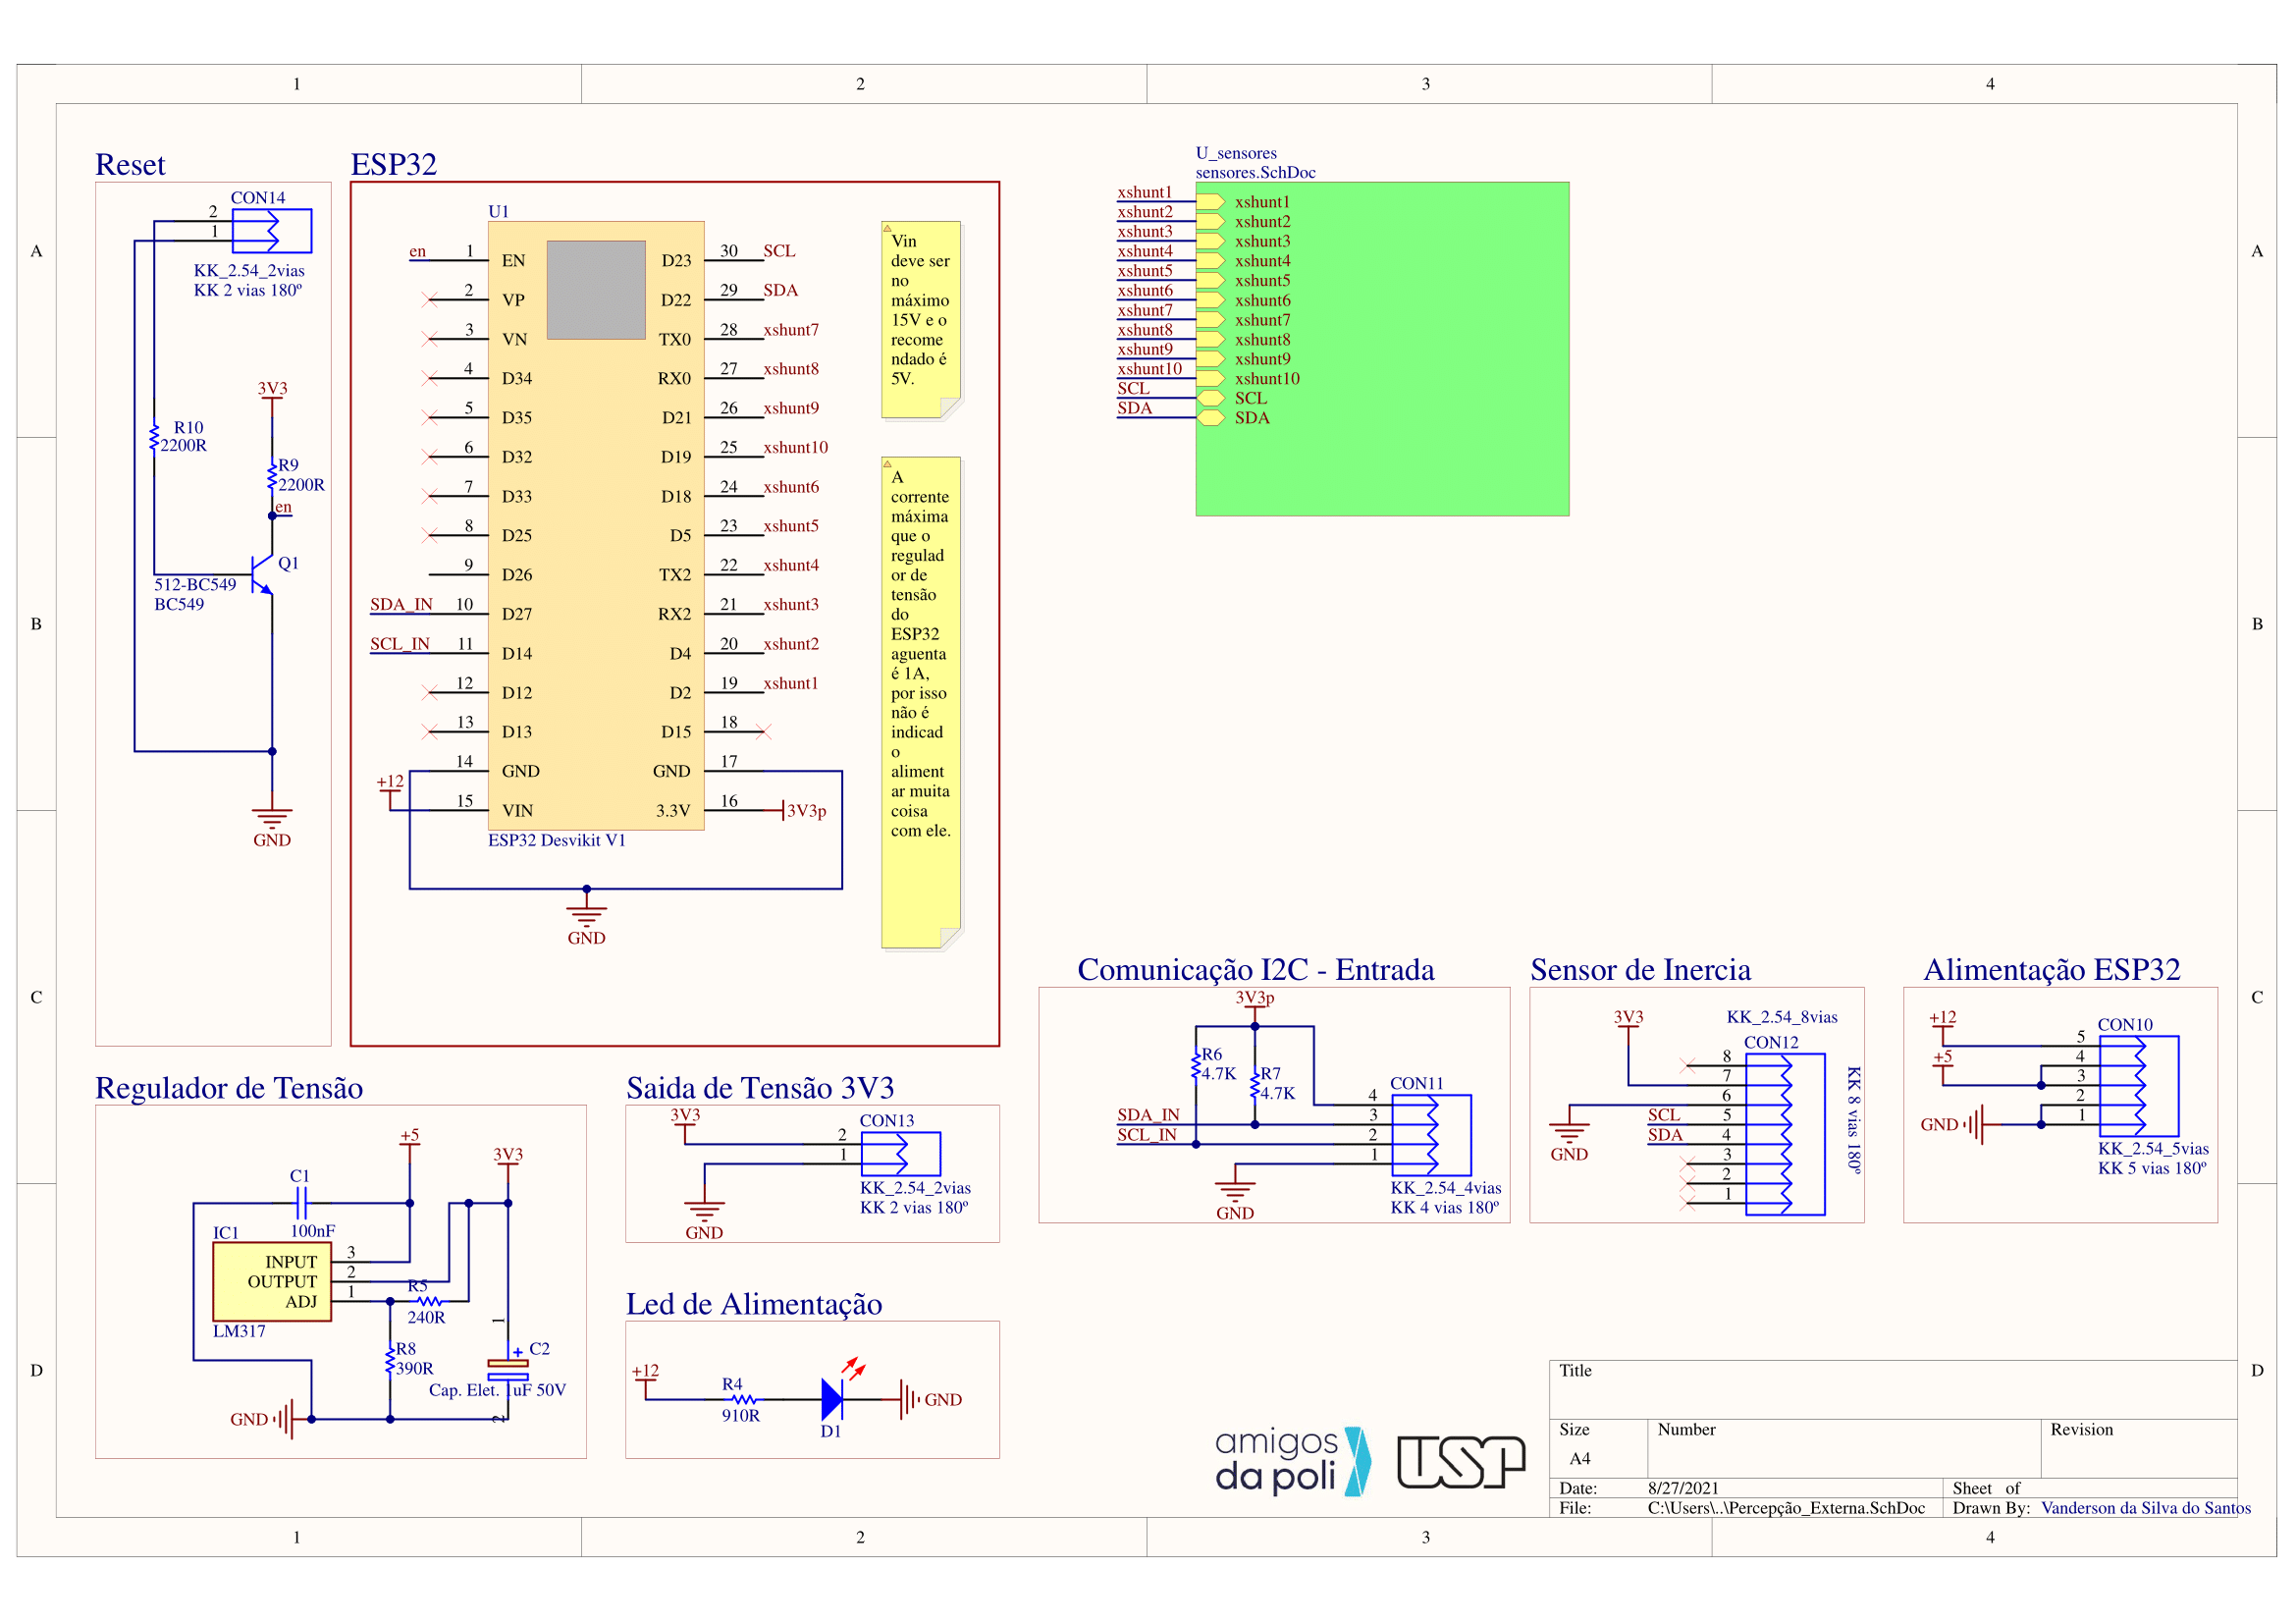
\includegraphics[width=17cm]{modulos/Percepção_Externa-1.png}
    \caption*{Fonte: Elaborado pelo autor no software Altium Design\cite{altium21} }
    \label{Protótipo placa de ## - Esquemático principal}
\end{figure}

\begin{table}[]
\caption{Componentes Utilizados na placa de Percepção Externa - Protótipo}
\centering
\begin{adjustbox}{width=\columnwidth,center}
\begin{tabular}{|c|c|c|c|c|}
\hline
Component                     & Description                                                    & Designator                                                    & Footprint                   & Quantity \\ \hline
100nF                       & CAP CER DISK 100NF   50V                                       & C1                                                            & CAP CER DISK 100NF   50V    & 1        \\ \hline
Cap. Elet. 1uF   50V        & Aluminum Organic   Polymer Capacitors 16volts 470uF ESR 10mohm & C2                                                            & Cap. Elet. 470uF 16V        & 1        \\ \hline
KK\_2.54\_6vias             & Conector KK 2.54mm 6   vias                                    & CON1, CON2, CON3,   CON4, CON5, CON6, CON7, CON8, CON9, CON15 & KK\_6vias\_180°             & 10       \\ \hline
KK\_2.54\_5vias             & Conector KK 2.54mm 5   vias                                    & CON10                                                         & KK\_5vias\_180°             & 1        \\ \hline
KK\_2.54\_4vias             & Conector KK 2.54mm 4   vias                                    & CON11                                                         & KK\_4vias\_180°             & 1        \\ \hline
KK\_2.54\_8vias             & Conector KK 2.54mm 8   vias                                    & CON12                                                         & KK\_8vias\_180°             & 1        \\ \hline
KK\_2.54\_2vias             & Conector KK 2.54mm 2   vias                                    & CON13, CON14                                                  & KK\_2VIAS\_180º             & 2        \\ \hline
LED 5MM RED                 & LED 5MM RED                                                    & D1                                                            & LED 5MM RED                 & 1        \\ \hline
LM317                       & Integrated Circuit                                             & IC1                                                           & TO254P467X1016X1971-3P      & 1        \\ \hline
BC549                       & TRANS NPN 30V 0.1A   TO-92                                     & Q1                                                            & TO92                        & 1        \\ \hline
RES 470R 1/4W   CARBON FILM & RES 470R OHM 1/4W 5\%   CARBON FILM                            & R4, R5, R8, R9, R10                                           & RES 470R 1/4W CARBON   FILM & 5        \\ \hline
4.7K                        & RES 4.7K OHM 1/4W 5\%   CARBON FILM                            & R6, R7                                                        & RES 4.7K 1/4W CARBON   FILM & 2        \\ \hline
microcontrolador            & microcontrolador com   moculo bluethoth e wifi                 & U1                                                            & ESP32\_Desvikit\_v1         & 1        \\ \hline

\end{tabular}
\end{adjustbox}
\centering
\caption*{Fonte: Elaborado pelo autor}
\label{table:voc}
\end{table}


\paragraph{Printed Circuit board (PCB)}

\begin{figure}[!ht]
    \centering
    \begin{minipage}{0.5\textwidth}
        \centering
        \caption{Protótipo Percepção Externa - PCB 2D}
        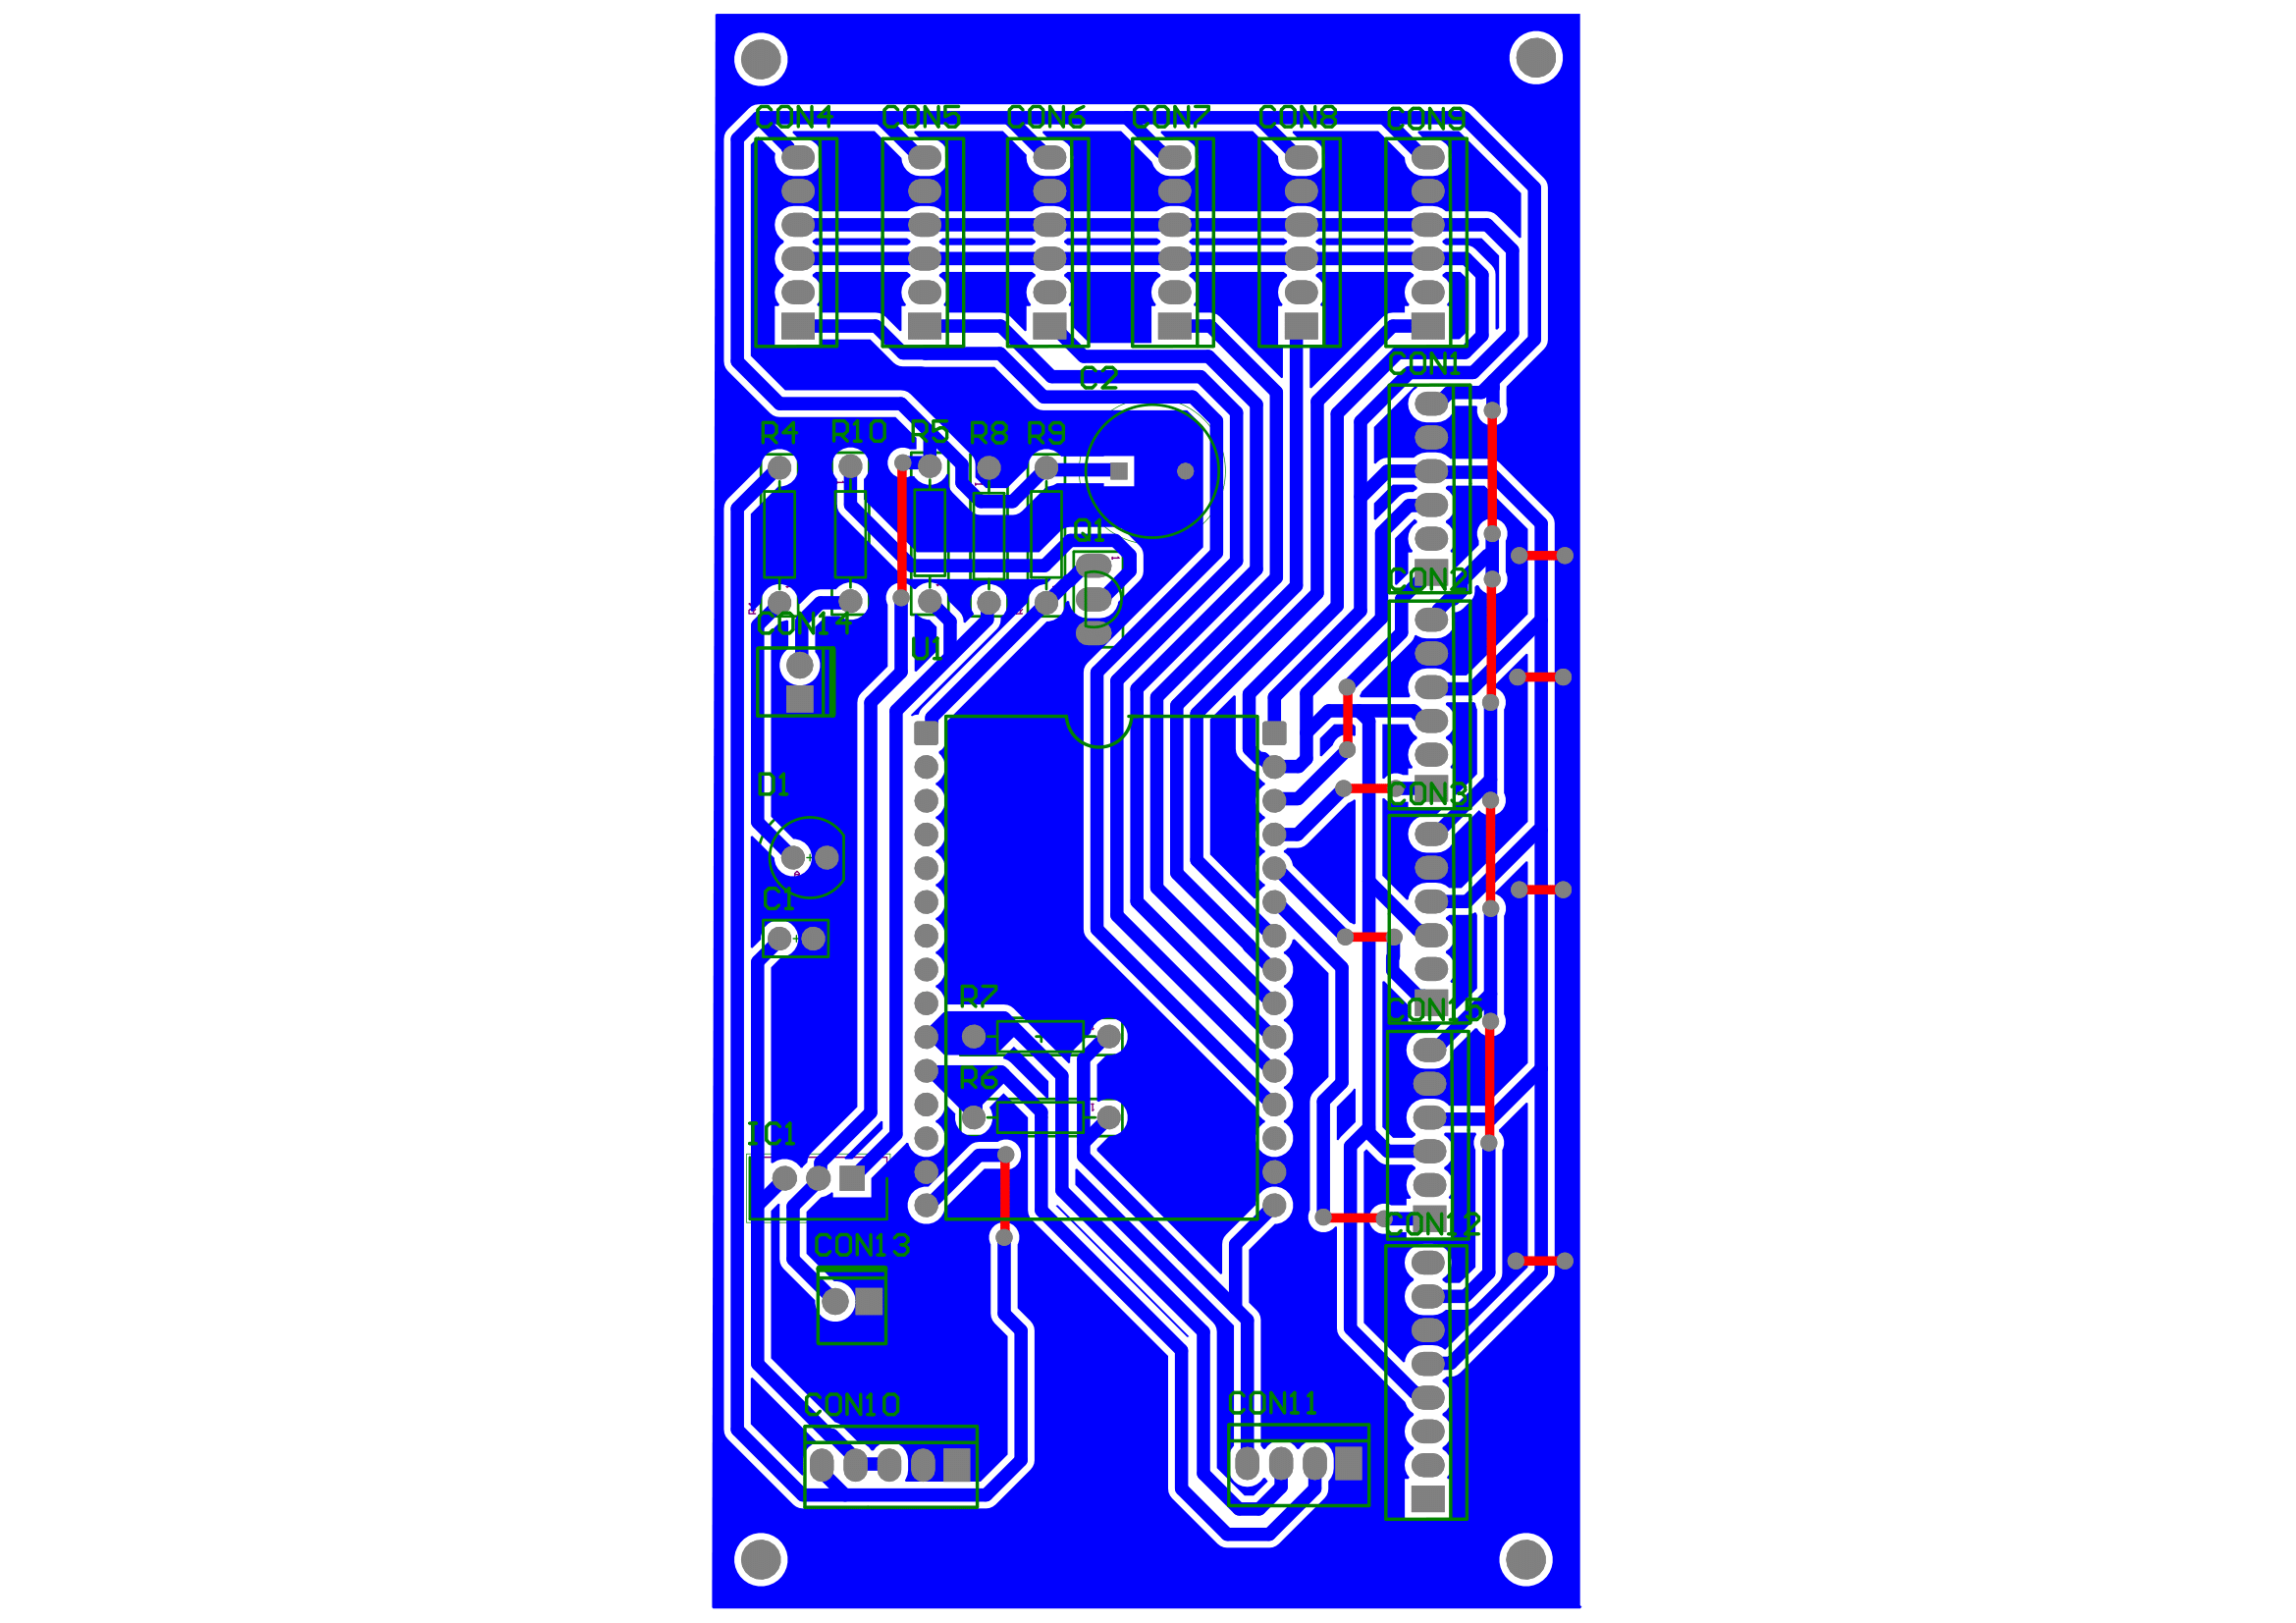
\includegraphics[width=1.03\textwidth]{modulos/Percepção_Externa-3.png} 
        \label{fig:figura1minipg}
    \end{minipage}\hfill
    \begin{minipage}{0.5\textwidth}
        \centering
        \caption{Protótipo Percepção Externa - PCB 3D }
        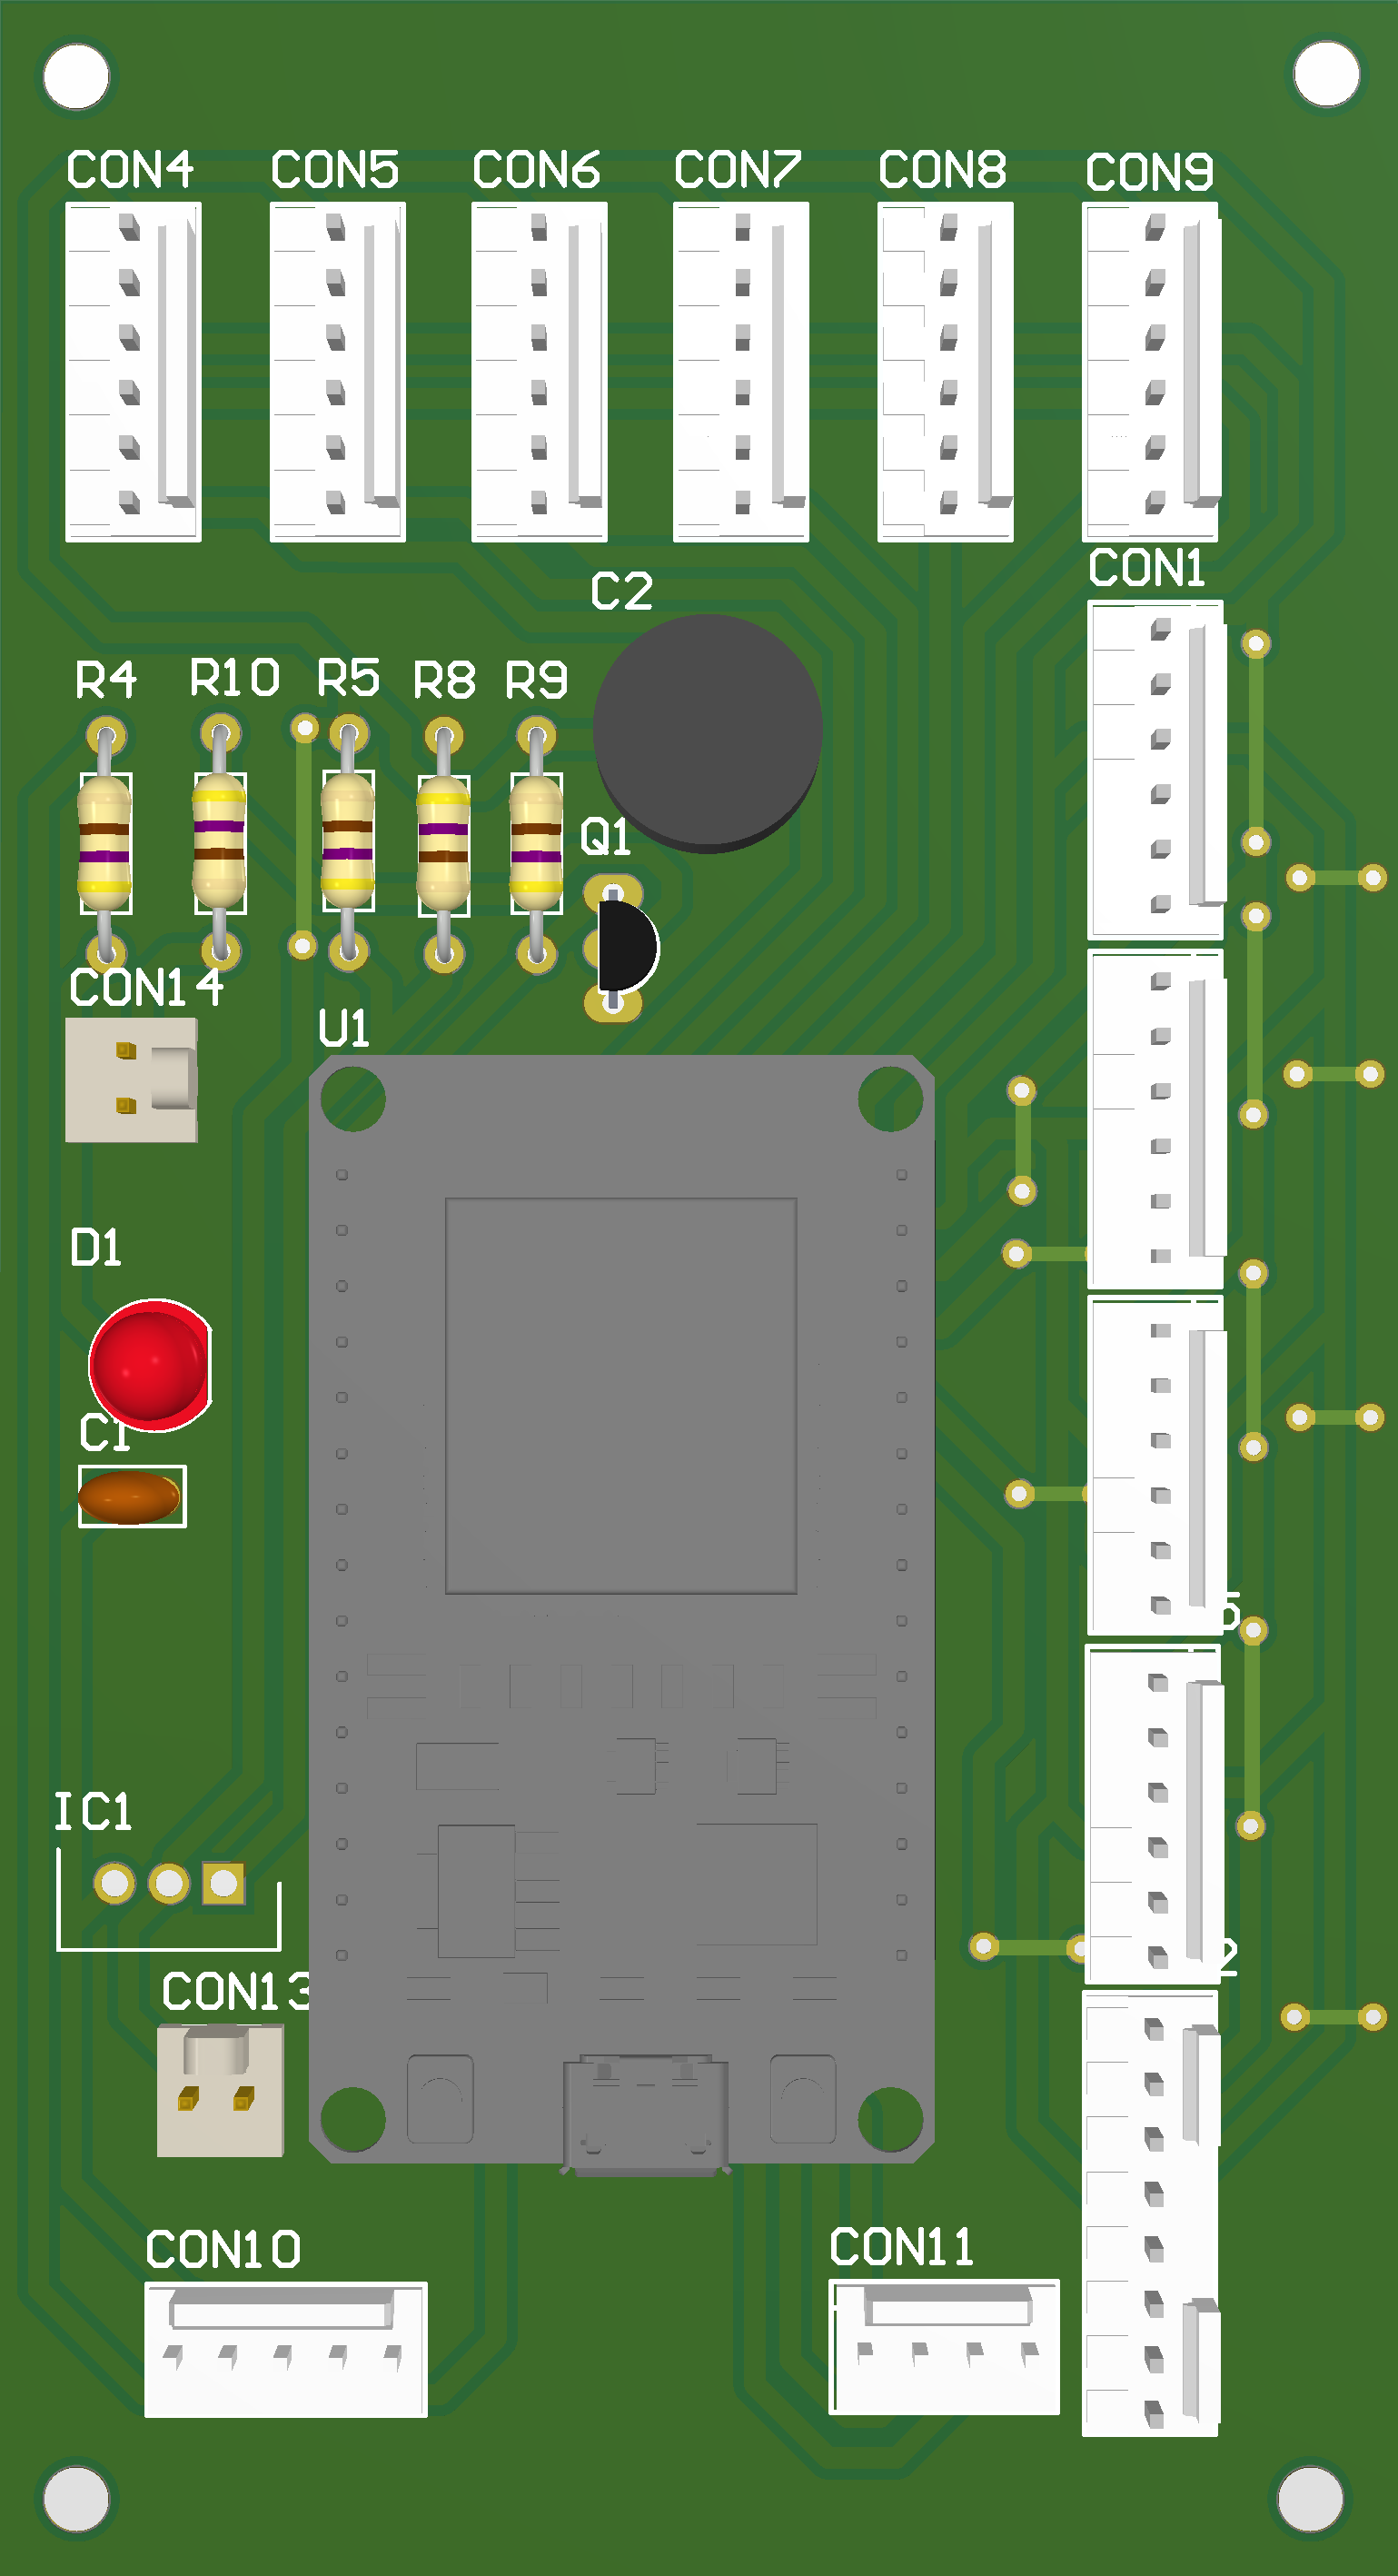
\includegraphics[width=0.4\textwidth]{modulos/Percepção_Externa.png} 
        \label{fig:figura1minipg}
    \end{minipage}\hfill
    
    \caption*{Fonte: Elaborado pelo autor no software Altium Design\cite{altium21} }
    \label{fig:figurasminipg}
\end{figure}

\begin{figure}[!ht]
    \centering
    \begin{minipage}{0.5\textwidth}
        \centering
        \caption{Protótipo Percepção Externa - Trilhas}
        \includegraphics[width=0.8\textwidth]{example-image-a} 
        \label{fig:figura1minipg}
    \end{minipage}\hfill
    \begin{minipage}{0.5\textwidth}
        \centering
        \caption{Protótipo Percepção Externa - Completa}
        \includegraphics[width=0.8\textwidth]{example-image-a} 
        \label{fig:figura1minipg}
    \end{minipage}\hfill
    
    \caption*{Fonte: Elaborado pelo autor }
    \label{fig:figurasminipg}
\end{figure}

%================================ PERCEPÇÂO OFICIAL ========================
\subsubsection{Oficial}

\paragraph{Esquemático}

\begin{figure}[h]
\centering
    \caption{placa de Percepção Externa - Esquemático principal }
    \centering % para centralizarmos a figura
    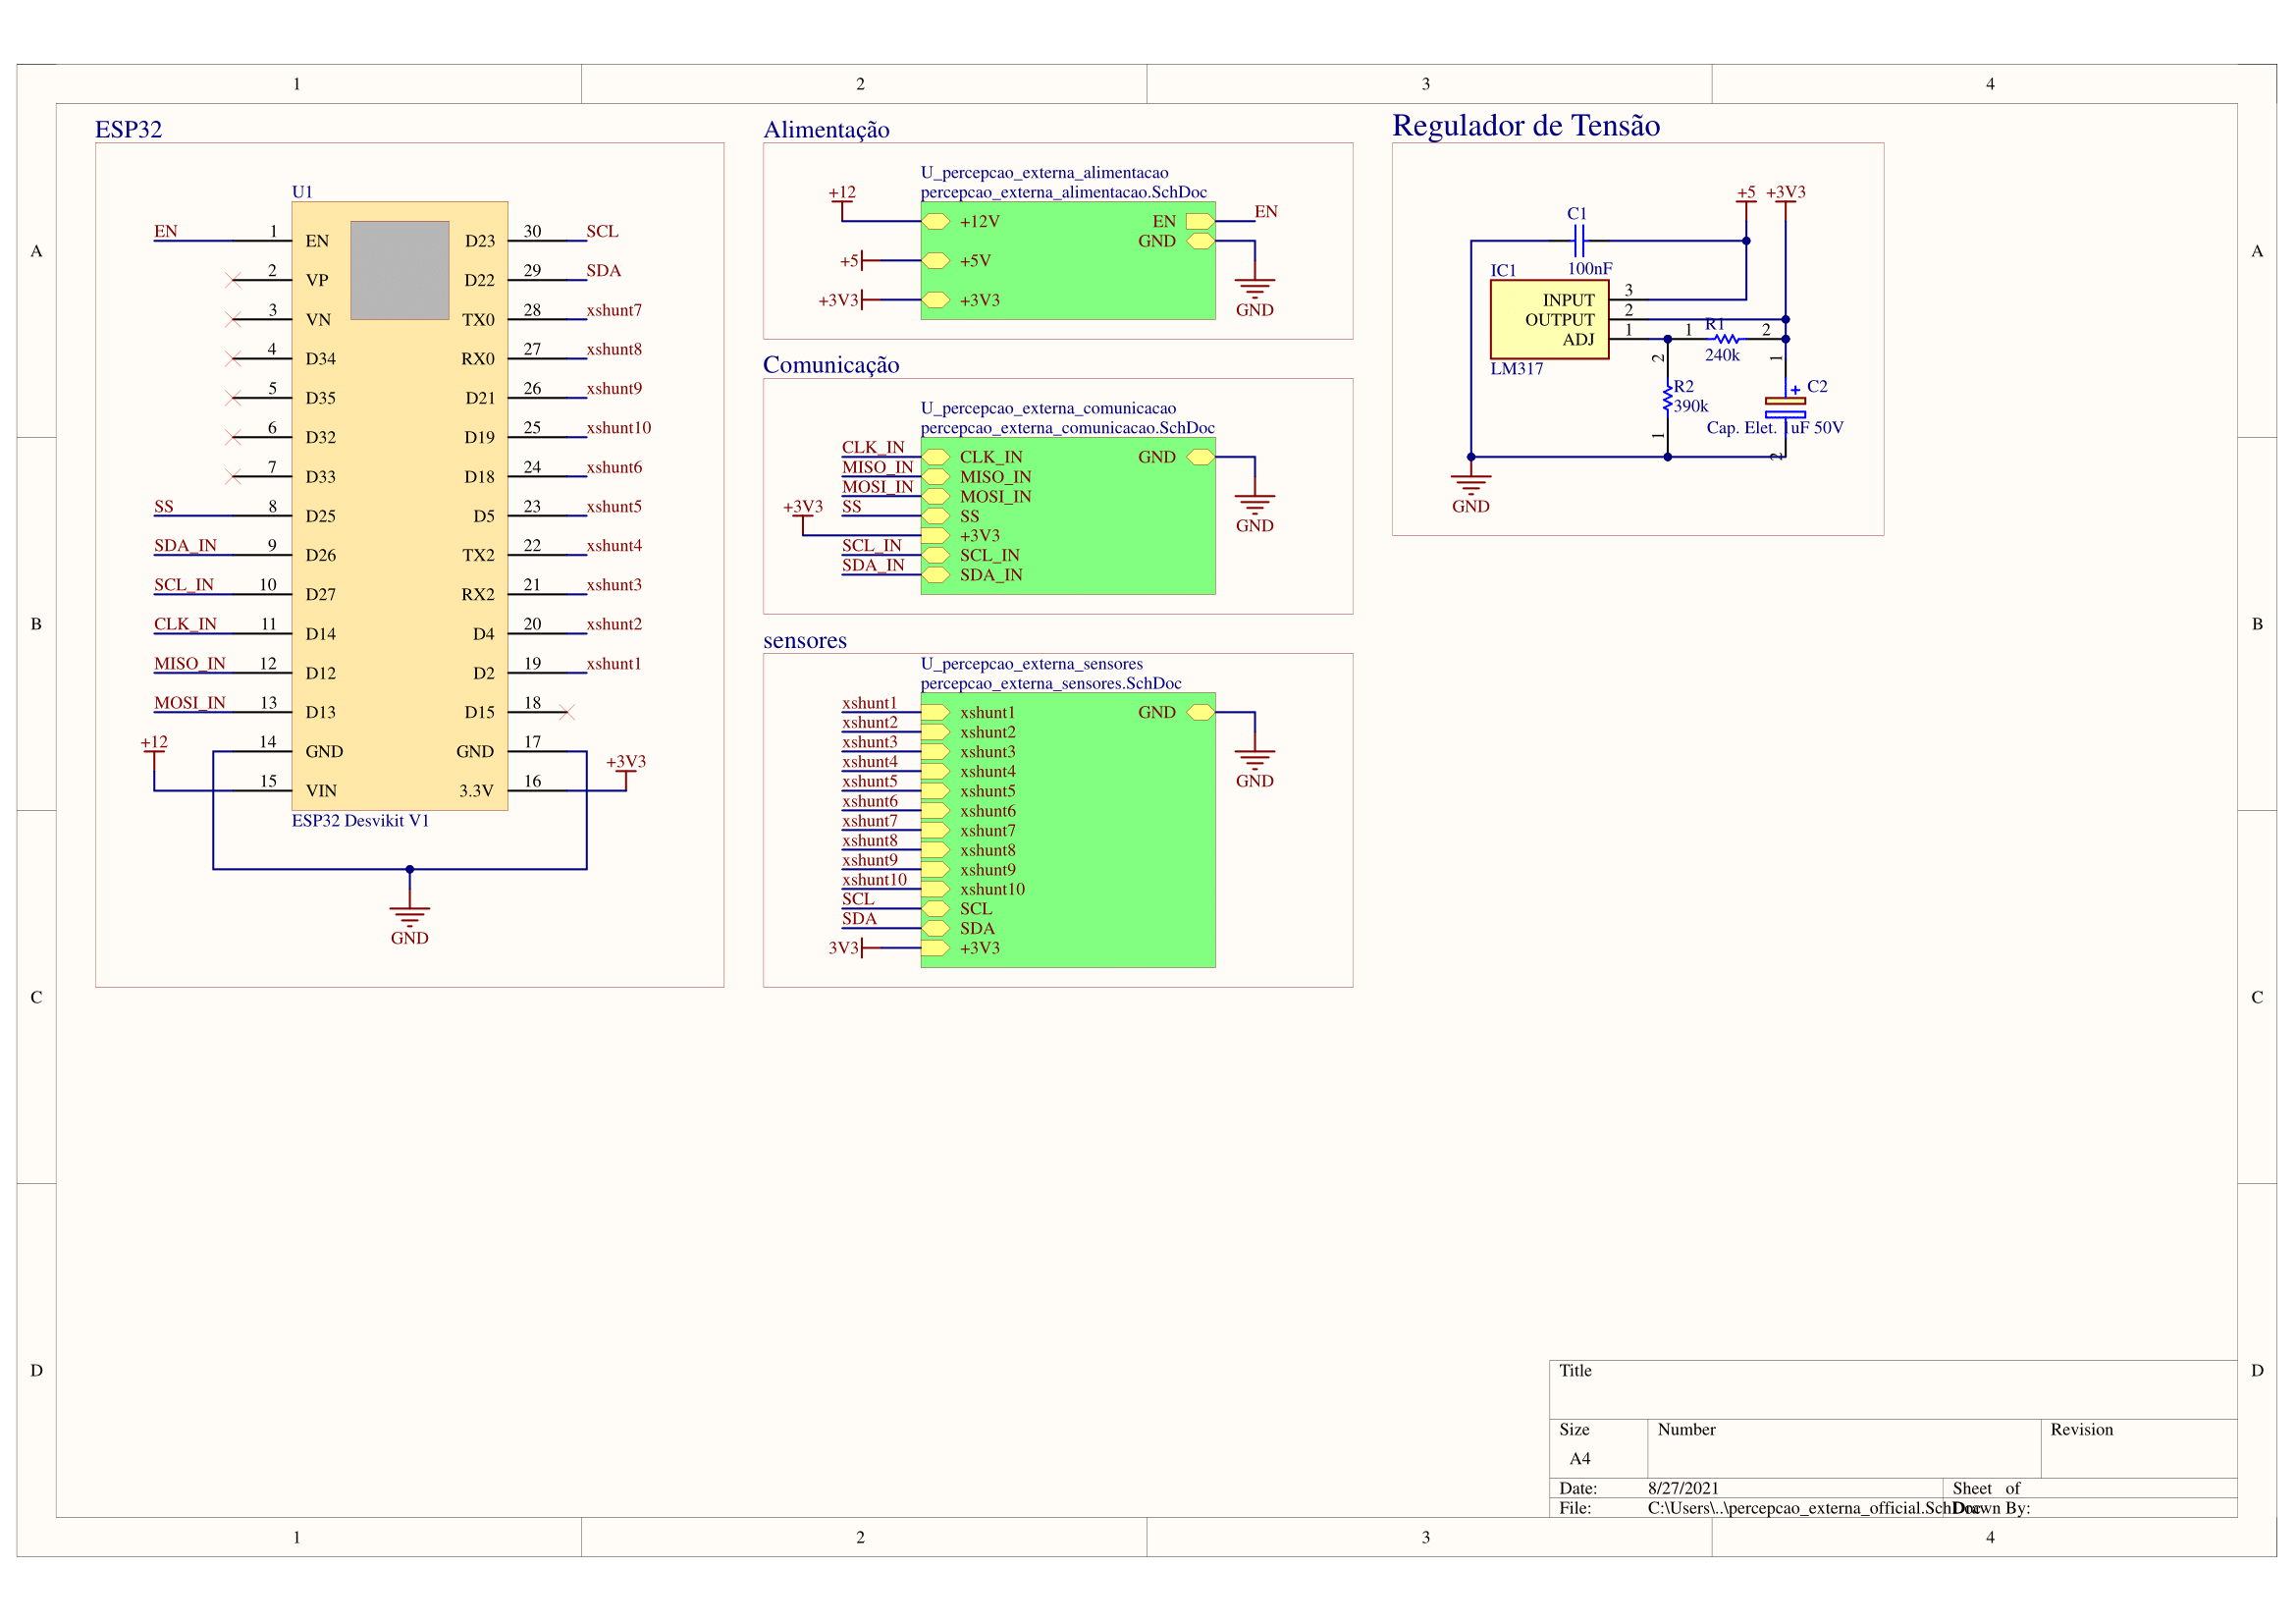
\includegraphics[width=17cm]{modulos/percepcao_externa_official-1.png}
    \caption*{Fonte: Elaborado pelo autor no software Altium Design\cite{altium21} }
    \label{Protótipo placa de ## - Esquemático principal}
\end{figure}

\begin{table}[]
\caption{Componentes Utilizados na placa de Percepção Externa}
\centering
\begin{adjustbox}{width=\columnwidth,center}
\begin{tabular}{|c|c|c|c|c|}

\hline
Component            & Description                                                    & Designator                                                                                                               & Footprint              & Quantity \\ \hline
100nF                & CAP CER DISK 10uF 50V                                          & C1                                                                                                                       & CAP CER DISK 10uF 50V  & 1        \\ \hline
Cap. Elet. 1uF   50V & Aluminum Organic   Polymer Capacitors 16volts 470uF ESR 10mohm & C2                                                                                                                       & Cap. Elet. 470uF 16V   & 1        \\ \hline
KK\_2.54\_2vias      & Conector KK 2.54mm 2   vias                                    & CON1, CON3, CON4                                                                                                         & KK\_2VIAS\_180º        & 3        \\ \hline
KK\_2.54\_6vias      & Conector KK 2.54mm 6   vias                                    & \begin{tabular}[c]{@{}l@{}}CON2, CON8, CON9,   CON10, \\ CON11, CON12, CON13, CON14, \\ CON15, CON16, CON17\end{tabular} & KK\_6vias\_180°        & 11       \\ \hline
KK\_2.54\_5vias      & Conector KK 2.54mm 5   vias                                    & CON5                                                                                                                     & KK\_5vias\_180°        & 1        \\ \hline
KK\_2.54\_4vias      & Conector KK 2.54mm 4   vias                                    & CON6                                                                                                                     & KK\_4vias\_180°        & 1        \\ \hline
KK\_2.54\_8vias      & Conector KK 2.54mm 8   vias                                    & CON7                                                                                                                     & KK\_8vias\_180°        & 1        \\ \hline
LED 3MM RED          & LED 3MM RED                                                    & D1                                                                                                                       & LED RED                & 1        \\ \hline
LM317                & Integrated Circuit                                             & IC1                                                                                                                      & TO254P467X1016X1971-3P & 1        \\ \hline
Trans BC817          & Transistor BJT NPN   BC817-25-7-F                              & Q1                                                                                                                       & SOT96P240X110-3N       & 1        \\ \hline
240k                 & RES 1206 5\%                                                   & R1                                                                                                                       & RESC3216X60N           & 1        \\ \hline
390k                 & RES 1206 5\%                                                   & R2                                                                                                                       & RESC3216X60N           & 1        \\ \hline
680R                 & Resistor                                                       & R3                                                                                                                       & RESC3216X60N           & 1        \\ \hline
2k2                  & Resistor                                                       & R4, R5                                                                                                                   & RESC3216X60N           & 2        \\ \hline
4k7                  & RES 1206 5\%                                                   & R6, R7                                                                                                                   & RESC3216X60N           & 2        \\ \hline
microcontrolador     & microcontrolador com   moculo bluethoth e wifi                 & U1                                                                                                                       & ESP32\_Desvikit\_v1    & 1        \\ \hline

\end{tabular}
\end{adjustbox}
\centering
\caption*{Fonte: Elaborado pelo autor}
\label{table:voc}
\end{table}


%================================ PERCEPÇÂO FIRMWARE ========================
\subsection{Firmware}

\end{document}